%version of 07-21-20

\chapter{Numbers I:
The Basics of Our Number System}
\label{ch:numbers-numerals}


\hfill
\begin{tabular}{l}
{\em Die Mathematik ist die K\"{o}nigin der Wissenschaften und die} \\
\hspace*{.25in}{\em Zahlentheorie ist die K\"{o}nigin der Mathematik.} \\
({\em Mathematics is the queen of the sciences and number theory} \\
\hspace*{.25in}{\em $\langle$often, ``arithmetic''$\rangle$ is the queen of mathematics.}) \\
%[La Math\'ematique est la reine des Sciences et la Th\'eorie des Nombres est la reine des Math\'ematiques.]
\hfill{\small
\begin{tabular}{l}
Karl Friedrich Gauss \\
Quoted in {\it Gauss zum Gedächtniss} (1856) by \\
\hfill Wolfgang Sartorius von Waltershausen 
\end{tabular} }
\end{tabular}

\index{von Waltershausen, Wolfgang Sartorius}
\index{Gauss, Karl Friedrich!Re: queen of science, queen of mathematics}


\section{Introducing the Three Chapters on Numbers}

\index{numbers}
Many, perhaps most, of us take for granted the brilliant notations that have been developed for the many arithmetic constructs that we use daily.  Our mathematical ancestors have bequeathed us notations that are not only perspicuous but also convenient for computing and for discovering and verifying new mathematical truths.  Several chapters in this text are devoted to sharing the elements of this legacy with the reader.  Three of these chapters focus on numbers themselves: the objects and how we represent them.
\begin{enumerate}
\item
The current chapter focuses on elementary concepts and techniques of reasoning relating to the most familiar objects of mathematical discourse, namely, the four families of numbers that underlie all of quantitative mathematics.
\medskip\item
Chapter~\ref{ch:numbers-advanced} extends this introductory material, by introducing some more advanced topics concerning numbers.  We look ``inward'' as we discuss important special classes of numbers which expose deep insights into the intrinsic nature of all numbers.  And, we
look ``outward'' as we reveal how numbers can ``encode'' structured data.  In this latter regard, we suggest some nonobvious implications of being able to perform such encodings.
\medskip\item
Chapter~\ref{ch:numerals} looks at {\it numerals}, the strings that we use to manipulate and analyze numbers.  Among a variety of representation-related topics, we discuss how much one can learn about intrinsics of various classes of numbers based only on the types of strings that we can use to name the numbers in the class.
\end{enumerate}
 \index{numerals} \index{numbers vs.~numerals}

\noindent \fbox{
\begin{minipage}{0.96\textwidth}
{\bf Explanatory note}.

\smallskip

Numbers and numerals embody what is certainly the most familiar instance of a very important dichotomy that pervades our intellectual lives: the distinction between objects and their names:

\smallskip

\hspace*{.2in}{\em Numbers are intangible, abstract objects.} \index{numbers!as objects}

\hspace*{.2in}{\em Numerals are the names we use to refer to and manipulate numbers.} 
\index{numerals!as names of numbers}

\smallskip

\index{numerals!operational}

\noindent
This is a critically important distinction!  You can ``touch'' a numeral: break it into pieces, combine two (or more) numerals via a large range of operations.  When the representations we use as numerals are {\em operational}, then you can {\em compute} using them.  Numbers are intangible abstractions, or, conceptualizations: you {\em reason} using numbers.
\end{minipage}
}

\section{A Brief Biography of Our Number System}
\label{sec:number-taxonomy}
\index{number system!biography}
\label{sec:numbers}

We begin our study of numbers and numerals with a short taxonomy of our number system.  Although we assume that the reader is familiar with the most common classes of numbers, we do spend some time highlighting important features of each class, partly, at least, in the hope of heightening the reader's interest in this most basic object of mathematical discourse.

We present the four most common classes of numbers in what is almost certainly the chronological order of their discovery/invention.
%{\Denis the quotation of Kronecker is done 3 times...}

\medskip

\noindent \fbox{
\begin{minipage}{0.96\textwidth}
{\bf Enrichment note}.

\smallskip

Did humans {\em invent} these classes of numbers to fill specific needs, or did we just {\em discover} their pre-existing selves as needs prompted us to search for them?  The great German mathematician Leopold Kronecker, \index{Kronecker, Leopold} as cited in \cite{Weber91} (on page 19), has asserted

\smallskip

\noindent
{\em Die ganzen Zahlen hat der liebe Gott gemacht, alles andere ist Menschenwerk.}

\smallskip

\noindent
[God made the integers, all else is the work of man].

\smallskip

\noindent
[Dieu a cr\'e\'e les nombres entiers, tout le reste est invention humaine].
\end{minipage}
}

\medskip

\index{number!integer} \index{number!zero ($0$)}
\index{number!negative} \index{$0$: zero} \index{zero ($0$)}

\noindent
A pleasing narrative can be fabricated to account for our multi-class system of numbers.  In the beginning, the story goes, we needed to count things (sheep, bottles of oil, weapons, \ldots), and the positive {\it integers} were discovered to serve this need.  As accounting practices matured, we needed to augment this class with the number zero ($0$) and with the negative integers.  The former augmentation (of zero) allowed Merchant $A$ to keep track of the inventory remaining after the last flask of wine is sold; the latter augmentation (of the negative numbers) allowed Merchant $A$'s banker to record $A$'s credit balance after taking a loan.  The class of integers was now complete---although a variety of special classes of integers remained to be discovered, motivated by reasons ranging from the religious to the intellectual.

\index{number!rational}

Moving on: As society matured, humans began to share materials that had to be subdivided---cloth, grain, etc.---rather than partitioned into discrete units.  We needed to invent the {\it rational numbers} to deal with such materials.  Happily for the mathematically inclined, the rational numbers could be developed in a manner that allowed one to view an integer as a special type of rational.  This meant that our ancestors could build upon the systems they had developed to deal with integers, rather than having to scrap those systems and start anew.

\bigskip

\noindent \fbox{
\begin{minipage}{0.96\textwidth}
{\bf Enrichment note}.

\smallskip

{\em The quest for {\em extendible} frameworks rather than isolated unrelated frameworks is a hallmark of mathematical thinking.}

One cannot overemphasize the centrality of this maxim to the success of mathematics over the millennia.
\end{minipage}
}

\bigskip

\index{Euclid} \index{Pythagoras}

\noindent
We now enter the realm of ``semi-recorded'' history in the West: our legacy from the Babylonians, the Egyptians, the Greeks, and others.  ``Practical'' mathematics was invented---and reinvented---to accommodate pursuits as varied as astronomy, commerce, navigation and architecture.  Our mathematical stalwarts, the integers and the rationals, were not adequate to deal with all of the measurements that we wanted to make, calculations that we wanted to do, structures that we wanted to design.  So, we approximated and ``fudged'' and got pretty much where we wanted to get.  The standard story at this point (at least in the West) is that the ancient Greeks began to try to systematize mathematical knowledge and practice.  The Greek mathematician and geometer Euclid,  and members of his school, verified---via one of the first {\em proofs} in recorded history---the uncomfortable fact that the lengths of portions of eminently buildable structures were not ``measurable''---in modern lingo, the lengths {\em were not rational}.  The poster child for this phenomenon was the {\em hypotenuse of the isosceles right triangle $T$ with unit-length legs}.  Thanks to the well-known theorem of the Greek mathematician Pythagoras, even schoolchildren nowadays know that the length of this eminently ``buildable'' line is $\sqrt{2}$.  What Euclid discovered is: {\em There is---provably!---no way to find integers $p$ and $q$ whose ratio is $\sqrt{2}$, the length of $T$'s hypotenuse.}\footnote{We present a version of Euclid's proof in Proposition~\ref{thm:sqrt(2)}.}

\bigskip

\index{The Pythagorean Theorem}

\noindent{\bf $\oplus$ Digression: {\em The Pythagorean Theorem}}.
The famed theorem of Pythagoras is widely known, at least informally.  We pause now to provide a {\em formal} statement of this seminal result and to provide a proof of the special case that relates to our current discussion of the square-root of $2$.  Quite aside from reviewing the Theorem's important content, this statement will provide the reader one more opportunity to ponder the ``music'' of mathematical discourse.

\medskip

\index{triangle} 
\index{triangle!right triangle}
\index{right angle} 
\index{right angle!$90^\circ$} 
\index{right angle!$90$ degrees}
\index{right angle!$\pi/2$ radians} 
\index{triangle!right triangle!side}
\index{triangle!right triangle!leg}
\index{triangle!right triangle!hypotenuse}
\index{triangle!isosceles triangle}
\index{triangle!isosceles triangle}

Let us be given a triangle $T$ with vertices $A$, $B$, and $C$.  Use the lefthand grey triangle in
Fig.~\ref{fig:unitsquare} as a model.
\begin{figure}[htb]
\begin{center}
       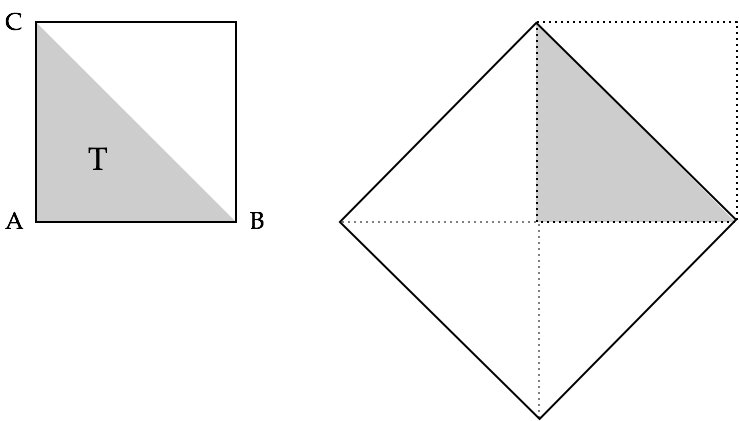
\includegraphics[scale=0.3]{FiguresArithmetic/UnitSquareSQRT2}
\caption{A pictorial schematic proof of The Pythagorian Theorem for the special case of an isosceles right triangle.
\label{fig:unitsquare}}
\end{center}
\end{figure}
Say that $T$ is a {\it right triangle}, meaning that one of its angles is a {\em right angle}, i.e., that its measure is $90^\circ$ (read: ``$90$ degrees'') or, equivalently, $\pi/2$ radians.  In our example, $T$'s right angle occurs at vertex $A$.  Because $T$ is a right triangle, the line from vertex $A$ to vertex $B$ and the line from vertex $A$ to vertex $C$ are called the {\em sides} (or the {\it legs}) of $T$, while the line from vertex $B$ to vertex $C$ is called the {\em hypotenuse} of $T$.  Triangle $T$ has a very special ``shape": it is {\em isosceles} meaning that its two sides /legs have the same length.  The grey triangle in Fig.~\ref{fig:unitsquare} is an isosceles right triangle.

\begin{theorem}[{\bf The Pythagorean Theorem}]
\label{thm:Pythagorean-thm}
Let $T$ be a right triangle whose two sides have respective lengths $s_1$ and $s_2$, and whose hypotenuse has length $h$.  Then
\[ h^2 \ = \ s_1^2 + s_2^2. \]
Consequently, when $T$ is an {\em isosceles} right triangle, then $h^2 = 2 s_1^2$.
\end{theorem}

The special case of the Pythagorean Theorem that deals with isosceles right triangles admits the very perspicuous proof presented pictorially in Fig.~\ref{fig:unitsquare}.  Follow along in the figure as we review this proof.

\smallskip

We focus first on the unit-side square $S$ on the left of the figure.  We partition $S$ by its diagonal into two unit-side isosceles right triangles, one grey and one white.  In this construction the diagonal of $S$ is the (shared) hypotenuse of the two triangles.  On the righthand side of Fig.~\ref{fig:unitsquare}, we use our partitioned version of $S$ to construct a new, bigger square, call it $\widehat{S}$, whose side-length is the hypotenuse-length of the grey triangle.  The dotted lines in the figure tell us how big $\widehat{S}$ is (measured by its area).
\begin{itemize}
\item
Square $S$ is unit-sided, hence has {\em unit area}, i.e., area $=1$.
\medskip\item
The grey triangle is (geometrically) half of $S$, hence has area $1/2$.
\medskip\item
Square $\widehat{S}$ is built from four copies of the grey triangle, hence has area $4 \cdot 1/2 \ = \ 2$.
\end{itemize}
Because the hypotenuse of the grey triangle is a side of an area-$2$ square, we have just proved the following special case of the Pythagorean Theorem\qed.\footnote{We generally signal the end of a proof via the symbol\qed, which can be read ``Q.E.D.", for ``{\em Quod Erat Demonstrandum}" [Latin for ``Which was to be proved"].}

\begin{prop}
\label{thm:unit-isosceles-PythThm}
The hypotenuse of the unit-side isosceles right triangle has length $\sqrt{2}$.
\end{prop}
  
\noindent \textbf{End of digression}

\bigskip

\index{Archimedes}

As part of the movement toward formalizing mathematics, the Sicily-based Greek mathematician and polymath Archimedes was systematically observing that squares are better approximations to circles than triangles are; regular pentagons are better approximations than squares; regular hexagons are better than pentagons; and so on.  Fig.~\ref{fig:approxcircle} illustrates this evidence.
\begin{figure}[htb]
\begin{center}
       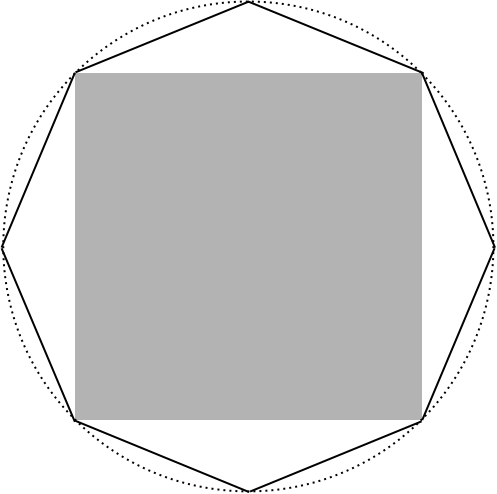
\includegraphics[scale=0.25]{FiguresArithmetic/ApproxCircle}
\caption{{\it Octagons approximate circles much better than squares do.}
\label{fig:approxcircle}}
\end{center}
\end{figure}
In fact, observed Archimedes, as the number of sides, $n$, in a regular polygon grows without bound (or, as we might say today, tends to infinity), each increase in $n$ brings a regular polygon closer to being a circle.

\medskip

\index{number!real}
\index{Descartes, Ren\'{e}}
\index{Cauchy, Augustin-Louis}
\index{Dedekind, Richard}
\index{numbers!real numbers}
\index{real numbers!non-rational}
\index{real numbers!irrational}

In order to pursue their respective observations to their completion, both Euclid and Archimedes would have had to leave the world of the rationals and enter the world of the {\it real numbers} (so named by the French mathematician-philosopher Ren\'{e} Descartes)---but this world did not yet exist!  It would take roughly two-thousand years from the days of Euclid and Archimedes before the real numbers were {\em formally} introduced to the world, by mathematical luminaries such as the early-19th-century French mathematician-scientist Augustin-Louis Cauchy and the late-19th-century German mathematician Richard Dedekind.  It turned out to be much easier to recognize instances of non-rational real numbers---better known as the {\it irrational} real numbers---than to formally delimit the entire family of such numbers.  Once again, happily, one could develop the real numbers in a way that allowed one to view a rational number as a special type of real number.  

\medskip

\index{polynomial} \index{polynomial!root}

During the millennia between the discoveries of Euclid, Archimedes, and their friends and the full development of the real numbers, mathematics was enriched repeatedly by the discovery of new conceptual structures.  One of these---polynomials and their roots---ultimately led to the final major subsystem of our number system.  In Chapter~\ref{sec:function}, we discussed the important notion of {\em function}.  Polynomials are a practically important class of functions that are delimited by the operations needed to compute them.  Specifically, an $n$-argument polynomial function---typically just called a {\it polynomial}---is a function $P(x_1, x_2, \ldots, x_n)$ whose values can be calculated using just the basic operations of arithmetic: addition/subtraction and multiplication/division.

\bigskip

\index{mutually inverse operations}

\noindent \fbox{
\begin{minipage}{0.96\textwidth}
{\bf Explanatory note}.

\smallskip

We pair the operations in this way because addition and subtraction are {\em mutually inverse
operations}, as are multiplication and division.  This means that one can undo an operation (say, an addition) by performing its inverse operation (in this case, a subtraction).  But {\em be careful:} one cannot undo multiplication by $0$.  
\end{minipage}
}

\bigskip

\index{polynomial!root}

A {\it root}  of a
polynomial (function) $P(x_1, x_2, \ldots, x_n)$ is an argument $\langle r_1, r_2, \ldots, r_n \rangle$ that causes $P$ to {\it vanish}, meaning that $P(r_1, r_2, \ldots, r_n) = 0$.  In Fig.~\ref{fig:sample-polys},
 \begin{figure}[htb]
\begin{center}
\begin{tabular}{|c|c|c|}
\hline
 & Polynomial $P(x)$ & Root(s) \\
\hline
1 &
$x+1$  &  $x= -1$ \\
2 &
$x-1$  &  $x= 1$ \\
3 &
$x^2 + 2x +1 = (x+1)^2$ & $x = -1$ \\ 
4 &
$x^2 - 2x +1 = (x-1)^2$ & $x = 1$ \\ 
5 &
$x^2 - 1$ & $x = 1$ and $x= -1$ \\
6 &
$x^2 + 1$ & {\em no real root} \\
7 &
$x^2 -2$  & $x = \sqrt{2}$ and $x = - \sqrt{2}$ \\
8 &
$x^2 + 2$ & {\em no real root} \\
\hline
\end{tabular}
\end{center} 
 \caption{A sampler of univariate polynomials.}
 \label{fig:sample-polys}
 \end{figure}
we illustrate a few sample {\em univariate}---i.e., {\em single-variable}---polynomials. \index{polynomial!univariate} \index{polynomial!single-variable}

\medskip

\noindent
There are lessons, both major and minor, to be gleaned from the examples in Fig.~\ref{fig:sample-polys}.
\begin{itemize}
\item
Entries 3 and 4 in the table illustrate that even simple polynomials can often be written in several different ways.  These entries illustrate also that roots can occur {\em with multiplicity:} one can view the value $x = -1$ as causing the polynomial $x^2 + 2x +1 = (x+1)\cdot (x+1)$ to vanish
in two ways---(1) by setting the lefthand factor $x+1$ to $0$ and (2) by setting the righthand factor $x+1$ to $0$.

\index{polynomial!root!multiplicity}

\medskip\item
Entries 5 and 7 illustrate that polynomials can have multiple distinct roots.

\medskip\item
Perhaps most importantly, entries 6 and 8 provide explicit, simple polynomials---whose expressions involve only positive integers---that fail to have any real roots!

\smallskip

The fact that the indicated polynomials have no real roots is immediate, because the square of a real number can never be negative. Hence, for instance, there is no positive integer $c$ such that $c^2 = -1$, or, equivalently, $c^2 + 1 = 0$.
\end{itemize}

\medskip

\index{al-Khw$\bar{\mbox{a}}$rizm$\bar{\mbox{i}}$, Muhammad ibn M$\bar{\mbox{u}}$s$\bar{\mbox{a}}$}

For both applied and purely intellectual reasons, there has always been considerable interest in developing techniques for finding the roots of polynomials.  Indeed, much seminal mathematics was developed in the quest for such techniques;\footnote{A giant in the development and transmission of this work was the $9$th-century mathematician and astronomer Muhammad ibn M$\bar{\mbox{u}}$s$\bar{\mbox{a}}$ al-Khw$\bar{\mbox{a}}$rizm$\bar{\mbox{i}}$.  We discuss his seminal contributions at greater length in Chapter~\ref{ch:arithmetic}.}~we study the topic at length in Section~\ref{sec:polynomials}.

\smallskip

\index{number!imaginary} \index{Descartes, Ren\'{e}} 
\index{imaginary number $i = \sqrt{-1}$}
\index{$i$: the imaginary unit}
\index{number!complex}

Closely related to this interest in a polynomial's roots was the considerable discomfort within the mathematical and technical world at the fact that the then-current number system---built upon the integers, the rationals, and the reals---was inadequate to the important task of providing roots for every polynomial.  The reaction to this deficiency was similar in kind to all earlier recognized deficiencies: a way was found to expand the number system!  Centuries would pass before mathematics developed adequately to find the needed expansion.  Once discovered, the expansion was based in the conception, in the $16$th century, of a new {\it imaginary} number, so designated by Descartes.\footnote{The term ``imaginary'' is reputed to be a derogation of these numbers that flouted tradition.}  This new number was named $i$ (for ``imaginary'') and was defined to be a root of the polynomial $P_{-1}(x) = x^2 +1$.  The number $i$ was evocatively often defined via the equation, $i = \sqrt{-1}$.  By keeping our extended arithmetic consistent with our former arithmetic, $-i$ also became a root of $P_{-1}(x)$.  When the imaginary number $i$ was added to the real number system, and the combination was blended
via the rules of arithmetic, the {\it complex number system} was born.

\smallskip

 \index{complex numbers!algebraically complete}
 
Thankfully, the imaginary number $i$ was the only totally new concept that was needed to mend the observed deficiency in the real numbers.  In formal terms, the complex numbers were shown to be {\it algebraically complete} in the sense expressed in the landmark {\it Fundamental Theorem of Algebra}:

 \index{Fundamental Theorem of Algebra}

\begin{theorem}[The Fundamental Theorem of Algebra]
Every polynomial of degree $n$ with complex coefficients has $n$ roots over the complex numbers.
\end{theorem}

The proof of the Theorem is beyond the scope of our introductory text, but the result is a notable milestone in our mathematical/technical culture.

\bigskip

Our historical tour is now complete, so we can---finally---begin to get acquainted with the several components our number system and the operations that bring each component to life in applications.

\section{Integers: The ``Whole'' Numbers}
\label{sec:integers}

\index{number!integer}
\index{number!integer!whole number}
\index{number!integer!counting number} \index{number!prime}
\index{pairing function}

The first class of numbers that most of us encounter comprise the {\it integers}, which are also referred to as the {\it whole numbers} or the {\em counting numbers}.  As suggested in our ``biography'' of our number system (Section~\ref{sec:number-taxonomy}), integers are certainly the numbers that our prehistoric ancestors employed in the earliest days of our species.  This section is devoted to exploring some of the basic properties of the class of integers.  The details we provide in Section~\ref{sec:primes} regarding the building blocks of the integers, the {\it prime numbers}, will prepare the reader for myriad applications of the integers, including important {\em (computer-)security-related} applications.  Our introduction to {\it pairing functions}, in Section~\ref{sec:pairing}, will open the door to myriad applications of the integers, which build on the ordering properties of these numbers, coupled with tools for encoding highly structured data as integers.

\subsection{The Basics of the Integers: The Number Line}
\label{sec:integer-number-line}
\index{number!the number line}
\index{number!integer!the number line}
\index{$\Z$: the set of all integers}
\index{$\N$: the set of nonnegative integers}
\index{$\N^+$: the set of positive integers}

We survey a number of the most important properties of the following three sets, which collectively comprise ``the integers.''
\begin{itemize}
\item
The set $\Z$ comprises {\em all integers}---the positive and negative integers plus zero ($0$).
\medskip\item
The set $\N$ comprises the {\em nonnegative integers}---the positive integers plus zero ($0$).
\medskip\item
The set $\N^+$ comprises the {\em positive integers}.
\end{itemize}
There is no universally accepted default when one refers to ``the integers'' with no qualifying adjective; therefore, we shall always be careful to indicate which set we are discussing at any moment---often by supplying the set-name: $\Z$ or $\N$ or $\N^+$.

\subsubsection{Natural orderings of the integers}
\label{sec:natural-orderings}
\index{less-than relation on numbers}
\index{less-than relation on numbers!the strict version: $<$}
\index{less-than relation on numbers!the weak version: $\leq$}
\index{greater-than relation on numbers}
\index{greater-than relation on numbers!the strict version: $>$}
\index{greater-than relation on numbers!the weak version: $\geq$}

Several essential properties of the sets $\Z$, $\N$, and $\N^+$ are consequences of the integers' behaviors under their natural {\em order} relations:
\begin{itemize}
\item
the two {\em less-than} relations:
  \begin{itemize}
  \item
the {\em strict} relation ($<$).  We articulate ``$a < b$'' as ``$a$ is (strictly) less than $b$'' or ``$a$ is (strictly) smaller than $b$.''
  \medskip\item
the {\em nonstrict}, or, {\em weak} relation ($\leq$).  We articulate ``$a \leq b$'' as ``$a$ is less than or equal to $b$'' or ``$a$ is no larger than $b$.''
  \end{itemize}
\index{$<$: the strict less-than relation} \index{$\leq$: the nonstrict/weak less-than relation}

\medskip\item
their {\em converses,} the {\em greater-than} relations:
  \begin{itemize}
  \item
the {\em strict} relation ($>$).  We articulate ``$a > b$'' as ``$a$ is (strictly) larger than $b$.''
  \medskip\item
the {\em nonstrict}, or, {\em weak} relation ($\geq$).  We articulate ``$a \geq b$'' as ``$a$ is greater than or equal to $b$'' or ``$a$ is no smaller than $b$.''
  \end{itemize}
\index{$>$: the strict greater-than relation}
\index{$\geq$: the nonstrict/weak greater-than relation}
\end{itemize}
One sometimes encounters {\em emphatic} versions of the strict relations: the notations $a \ll b$ and $a \gg b$ indicate that $a$ is, respectively, {\em much smaller than} or {\em much larger than} $b$.  Usually, the qualifier ``much" is not quantified, but sometimes it is.
\index{$\ll$: the emphatic strict less-than relation}
\index{$\gg$: the emphatic strict greater-than relation}

\smallskip

The reader will note throughout the text that order relations within a number system are among one's biggest friends when reasoning about numbers.  \index{number!ordering of numbers}

\subsubsection{The order-related laws of the integers}
\label{sec:order-laws}

\index{number!integer!total order} \index{integer!total order}
\index{number!integer!linear ordering} \index{integer!linear ordering}

\noindent{\small\sf A. Total order and the Trichotomy Laws}

The sets $\Z$, $\N$, and $\N^+$ are {\em totally ordered}, also termed {\em linearly ordered}

\smallskip

\index{number!integer!Trichotomy Laws} 
\index{integer!Trichotomy Laws} \index{Trichotomy Laws!integers}

These facts are embodied in the {\em Trichotomy Laws for integers}.

\medskip

{\it The Trichotomy Laws for integers}.

\smallskip

(i)
{\it For each integer $a \in \Z$, precisely one of the following is true.}

\hspace*{.2in} $a$ equals $0$: $(a=0)$ \ \ \ \ \ \
 $a$ is {\em positive}: $(a>0)$ \ \ \ \ \ \
 $a$ is {\em negative}: $(a<0)$

\smallskip

(ii)
{\it For each integer $a \in \N$, precisely one of the following is true.}

\hspace*{.2in} $a$ equals $0$: $(a=0)$ \ \ \ \ \ \ $a$ is {\em positive}: $(a>0)$

\smallskip

(iii)
{\it For each integer $a \in \N^+$:}

\hspace*{.2in} $a$ is {\em positive}: $(a>0)$

\bigskip

Consequently:
\smallskip

\index{number!the number line}

(i')
$\Z$ can be visualized via the ($2$-way infinite) number line:
\[ \ldots, -3, \  -2, \ -1, \ 0, \ 1,\  2, \ldots \]

\smallskip

(ii')
$\N$ can be visualized via the ($1$-way infinite) number line:
\[  0, \ 1, \ 2, \ 3, \ldots \]

\smallskip

(iii')
$\N^+$ can be visualized via the ($1$-way infinite) number line:
\[  1, \ 2, \ 3, \ldots \]

\medskip

The Trichotomy Laws can be expressed using arbitrary pairs of integers, rather than insisting that one of the integers be zero.  For the set $\Z$, for instance, this version of the Laws takes the following form:

\smallskip

{\it For any integers $a, b \in \Z$, precisely one of the following is true.}

\hspace*{.2in} $a$ equals $b$: $(a=b)$ \ \ \ \ \ \
 $a$ is less than $b$: $(a<b)$ \ \ \ \ \ \
 $a$ is greater than $b$: $(a>b)$

\medskip

\noindent{\small\sf B. Well-ordering}

\smallskip

The sets $\N$ and $\N^+$ are {\it well-ordered}.
\index{number!nonnegative integers!well-ordering} \index{nonnegative integers!well-ordering}
\index{number!positive integers!well-ordering} \index{positive integers!well-ordering}

\medskip

\noindent
{\it The Well-ordering law for nonnegative and positive integers}.

{\it Every subset of $\N$ or of $\N^+$ has a smallest element (under the ordering $<$).}

\bigskip

We digress momentarily to point out a nontrivial consequence of the well-ordering of the positive integers.  We have already seen this consequence stated as Proposition~\ref{thm:build-a-set}, which we now have the tools to prove.

\medskip

\noindent
{\bf Proposition}~\ref{thm:build-a-set} [{\sc compact form}].
{\em The set $S$ of Proposition~\ref{thm:build-a-set} contains $\N^+$.}


\begin{proof}[Proposition~\ref{thm:build-a-set}]
Say, for the sake of contradiction, that the set $S$ specified in the statement of the proposition does not contain every positive integer.  By the Well-Ordering Principle, there must then be a {\em smallest} positive integer, call it $k$, that does not belong to $S$.  Clearly, $k>1$, because the proposition asserts that $1 \in S$.  Therefore, the number $k-1$ is a positive integer. Moreover, $k-1$, being smaller than $k$, belongs to $S$.

But now, by definition, of $S$, we see that $(k-1)+1 = k$ {\em does belong to} $S$.

Thus, the assumption that $S$ does not contain every positive integer leads to a contradiction.  We infer that Proposition~\ref{thm:build-a-set} is true.  \qed
\end{proof}

\smallskip

\noindent{\small\sf C. Discreteness}

\smallskip

The set $\Z$ is {\it discrete}.
\index{number!integer!discreteness} \index{integer!discreteness}

\medskip

\noindent
{\it The discreteness of the integers.}

{\it For every integer $a \in \Z$, there is no integer between $a$ and $a+1$; i.e., there is no $b \in \Z$ such that $a < b < a+1$.}

\medskip

\noindent{\small\sf D. The law of ``between-ness''}

\smallskip

{\it The ``between-ness'' law} for the set $\Z$:
\index{number!integer!''between-ness'' law} \index{integer!''between-ness'' law}

\smallskip

\noindent
{\it For any integers $a, b \in \Z$, there are finitely many $c \in \Z$ such that $a < c < b$.}

\smallskip

\noindent
Any such $c$ lies {\em between} $a$ and $b$ along the number line, whence the name of the law.

\medskip

\noindent{\small\sf E. The cancellation laws}

\index{number!integer!cancellation laws} \index{integer!cancellation laws}

There are two {\it cancellation laws} for the set $\Z$, one for the operation of addition and one for the operation of multiplication.

\medskip

\noindent
{\it The cancellation law for addition}.

{\it For any integers $a, b, c \in \Z$, if $a+c = b+c$, then $a = b$.}
\index{number!integer!cancellation laws!addition} \index{integer!cancellation laws!addition}

\smallskip

\noindent
{\it The cancellation law for multiplication}.

{\it For any integers $a, b \in \Z$ and $c \in \Z \setminus \{0\}$, if $a \cdot c = b \cdot c$, then $a = b$.}
\index{number!integer!cancellation laws!multiplication} 
\index{integer!cancellation laws!multiplication}

\smallskip

\noindent
The cancellation laws provide limited versions of the algebraic notion of mutually inverse arithmetic operations (Section~\ref{sec:binary-operators}).
\index{arithmetic operations!mutually inverse operations}


\subsection{Divisibility: Quotients, Remainders, Divisors}
\label{sec:divisibility}
\index{divisibility} \index{integers!divisibility}

This section is devoted to studying the fundamental relation of {\em divisibility} between two integers.  Let $m, n \in \N$ be nonnegative integers.  We use any of the following notations to assert the existence of a positive integer $q$ such that $n = q \cdot m$.
\index{number!integer!divisor}
\index{number!integer!divisibility} \index{$m \mid n$: $m$ divides $n$}
\begin{itemize}
\item
$m$ {\it divides} $n$
\medskip\item
$m$ {\it is a divisor of} $n$
\medskip\item
$n$ {\it is divisible by} $m$
\medskip\item
$m \mid n$.
\end{itemize}
This section is devoted to studying the possible {\it divisibility} relations between integers $m$ and $n$.  We begin by noting some general facts.
\begin{itemize}
\item
{\em Every integer $m$ divides $0$.}

\smallskip

This is because of the universal equations $m \cdot 0 = 0 \cdot m = 0$.   The same equations verify that $0$ {\em does not divide any integer.}

\medskip\item
{\em $1$ divides every integer.}

\smallskip

This is because of the universal equation $1 \cdot m = m$.
\medskip\item
{\em Every nonzero integer divides itself.}

\smallskip

This is because of the universal equation $m \cdot 1 = m$.
\end{itemize}

Some nonzero integers have many distinct divisors, while some have very few.  Consider, for illustration, the first twelve positive integers.
\[ \begin{array}{|c|c|}
\hline
\mbox{Number} & \mbox{Divisors} \\
\hline
\hline
1  &  \{ 1 \} \\
2  &  \{ 1, 2 \} \\
3  &  \{ 1, 3 \} \\
4  &  \{ 1, 2, 4 \} \\
5  &  \{ 1, 5 \} \\
6  &  \{ 1, 2, 3 \} \\
7  &  \{ 1, 7 \} \\
8  &  \{ 1, 2, 4, 8 \} \\
9  &  \{ 1, 3, 9 \} \\
10  & \{ 1, 2, 5, 10 \} \\
11  & \{ 1, 11 \} \\
12  & \{ 1, 2, 3, 4, 6, 12 \} \\
\hline
\end{array}
\]
All nonzero integers (except for $1$) have at least two divisors, $1$ and themselves.  The ``sparsely divisible'' integers that have only these two divisors are called {\it primes} or {\it prime  integers} or {\it prime numbers}.  We study these ``building blocks of the positive integers'' in more detail in Section~\ref{sec:primes}.  While there is, indeed, much of interest to discuss about prime numbers, the {\it composite}---or, nonprime---integers are also quite interesting, particularly, when we focus of {\em pairs} of integers.  The next section looks at the defining property of composite integers, namely, {\em divisibility}.

\index{numbers!integers!prime} \index{numbers!integers!composite} 

\medskip

\index{Euclid!Euclidean division}

In order to better understand the fundamental concept of divisibility, we must broaden our perspective somewhat and consider the notion of {\em Euclidean division}, i.e., division with remainders.  The notion of ``perfect'' divisibility that we have been discussing thus far is the special case in which the remainder is $0$.  The next subsection studies Euclidean division; the remainder of this section investigates the ramifications of ``perfect'' divisibility.

\subsubsection{Euclidian division}
\label{sec:euclidian}
\index{Euclid!Euclidean division} \index{Euclid} \index{quotient} \index{remainder}

Divisibility is not always perfect: Given a pair of integers, neither needs be an integer multiple of the other.  As we learned in elementary school, if an integer $m > 0$ does not ``evenly'' divide an integer $n > m$, then we are left with a ``remainder'' when we attempt to divide $n$ by $m$.  {it Euclidean}  {\it division}---so named for the Greek mathematician Euclid, whose writings introduced the process in the West---is the process of producing, given integers $m >0$ and $n >m$, an integer {\it quotient} $q$ and an integer {\it remainder} $r$ (where $0 \leq r < m$) such that $n = q \cdot m + r$.  The process of Euclidean division always succeeds, in the following strong sense.

\begin{theorem}[The Division Theorem]
\label{thm:division-thm}
Given any integers $n$ and $m > 0$, there exists a unique pair of integers $q$ and $r$, with $0 \leq r < m$ such that
\begin{equation}
\label{eq:euclid-division}
n \ = \ q \cdot m + r.
\end{equation}
\end{theorem}

\begin{proof}
We first prove that a result-pair $\langle q, r \rangle$, as described in the Proposition, exists for each argument-pair $\langle m, n \rangle$.  Then we prove that the result-pair is unique.

\medskip

\noindent {\em There exists at least one argument-pair}.
Given any argument-pair $\langle m, n \rangle$, let $N_{m,n}$ be the set of all integers of the form $(n - a \cdot m)$ for some integer $a$.  Symbolically,
\[ N_{m,n} \ \eqdef \ \{ (n - a \cdot m) \ \ | \ \  \mbox{ both } \  a,  \
(n - a \cdot m) \in \N  \}
\]
Each such set $N_{m,n}$ is a nonempty set of nonnegative integers: the nonemptiness follows because $n \in N_{m,n}$ (via the case $a=0$).  By the Well-ordering law, $N_{m,n}$ contains a (perforce, unique) {\em smallest} element.  Let us denote this smallest element by $r$, and let us denote by $a_r$ the value of $a$ that yields $r$; i.e.,
\[ n - a_r \cdot m \ = \ r.  \]
We complete this section of the proof, we need show that $r < m$.  Say, for contradiction, that $r = m+r'$ for some $r' \in \N^+$.  We then find
\[ n - (a_r +1)  \cdot m \ = \ r -m \ = r' \]
to be an element of $N_{m,n}$ that is strictly smaller than $r$.  This contradiction completes the first part of the proof.

\medskip

\noindent {\em 2. There exists at most one argument-pair}.
Turn now to the issue of uniqueness.  Say, for the sake of contradiction, that there exists an argument-pair $\langle m, n \rangle$, for which there exist distinct result-pairs $\langle q_1, r_1 \rangle$ and $\langle q_2, r_2 \rangle$.  We therefore have
\begin{equation}
\label{eq:euclid-unique}
n \ = \ q_1 \cdot m + r_1 \ = \ q_2 \cdot m + r_2,
\end{equation}
where both $r_1$ and $r_2$ satisfy the inequalities $0 \leq r_1, r_2 <m$.  We consider two cases.
\begin{itemize}
\item \textbf{Case 1.}
Assume first that $r_2 = r_1$.  In this case, the equations of (\ref{eq:euclid-unique}) tell us that
\[ q_1 \cdot m \ = \ q_2 \cdot m. \]
The cancellation law for multiplication then tells us that $q_1 = q_2$.  Therefore, the allegedly distinct result-pairs are, in fact, identical.

\medskip\item \textbf{Case 2.}
If $r_2 \neq r_1$, then say, with no loss of generality, that $r_2 > r_1$.  In this case, the equations of (\ref{eq:euclid-unique}) tell us that
\[ (q_1 - q_2) m \ = \ r_2 - r_1 . \]
Because the righthand quantity is positive, so also must be the lefthand quantity; i.e., $q_1 > q_2$ because $r_2 > r_1$.

On the one hand, the lefthand quantity, $(q_1 - q_2) m$, is no smaller than $m$.  This is because $q_1$ and $q_1 > q_2$ are integers.  On the other hand, the lefthand quantity, $r_2 - r_1$ is strictly smaller than $m$.  This is because $r_1 \geq 0$ so that $r_2 - r_1$ is no larger than $r_2$.
\end{itemize}
Both of the relevant cases thus lead to contradictions, so we must conclude that no argument-pair gives rise to more than one result-pair.  \qed
\end{proof}


\subsubsection{Divisibility, divisors, {\sc gcd}s}
\label{sec:divisibility+GCD}

We begin to study the several important aspects of integer divisibility by considering a variety of simple, yet significant, consequences of an integer $n$'s being divisible by an integer $m$.  We leave the following applications of the basic definitions as exercises for the reader.

\begin{prop}.
\label{thm:basic-divisibility}
\begin{enumerate}
\item
If $m$ divides $n$, then $m$ divides all integer multiples of $n$. That is: If $m$ divides $n$, then $m$ divides $cn$ for all integers $c$.

\medskip\item
The relation ``divides'' is {\em transitive}.\footnote{See Chapter~\ref{sec:order-relation}.}  Specifically, if $m$ divides $n$ and $n$ divides $q$ for some integer $q$, then $n$ divides $q$.

\medskip\item
The relation ``divides'' {\em distributes} over addition.\footnote{We use the term ``distributes'' in the sense of the Distributive Law; see Section~\ref{sec:Arithmetic-Laws}.}  That is, if $m$ divides $n$ and $m$ divides $(n+q)$ for some integer $q$, then $m$ divides $q$.
%\footnote{Hint: $\displaystyle \frac{n+q}{m} \ =  \ \frac{n}{m} + \frac{q}{m}$.}

\medskip\item 
For any integer $c \neq 0$,
\[ \left[m \mbox{ divides } n \ \ \mbox{ if, and only if, } \ \ cm \mbox{ divides } cn \right]. \]
\end{enumerate}
\end{prop}

The following result follows from the preceding facts.

\begin{prop}
\label{thm:m-commondivisor-n-q}
Given integers $m$, $n$, and $q$, if $m$ divides both $n$ and $q$, then $m$ divides all linear combinations of $n$ and $q$; i.e., $m \mbox{ divides } (sn + tq)$ for all integers $s$ and $t$.
\end{prop}

\begin{proof}
Because $m$ divides both $n$ and $q$, 
there exist integers $k_1$ and $k_2$ such that $k_1 \cdot m = n$ and $k_2 \cdot m = q$.  By the distributive law, we therefore have:
\[ (k_1 \cdot s \ + \ k_2 \cdot t)m \ = \ sn+tq \]
for any $s$ and $t$.  \qed
\end{proof}

\index{greatest common divisor} \index{{\sc gcd}: greatest common divisor}
Among the common divisors of integers $n$ and $q$, a particularly significant one is their {\em greatest common divisor}, which is the {\em largest} integer that divides both $n$ and $q$.  We abbreviate ``greatest common divisor'' by {\sc gcd}, and we write
\[ m \ = \ \mbox{\sc gcd}(n, q) \]
to identify an integer $m$ as the {\sc gcd} of $n$ and $q$.

\smallskip

We are finally ready for our first major result about integer division and divisors.
\index{B\'{e}zout, Etienne}

\begin{prop}[B\'{e}zout's identity]
\label{thm:gcd-n-linear}
For positive integers $n$ and $q$, {\sc gcd}$(n, q)$ is the smallest positive linear combination of $n$ and $q$.

\medskip

\noindent
Stated alternatively, the following two statements both hold.
\begin{itemize}
\item
For any positive integers $n$ and $q$, there exist integers $s_0$ and $t_0$, not necessarily positive, such that $s_0 n + t_0 q \ = \ \mbox{\sc gcd}(n, q)$.
\item
For all integers $s$ and $t$, not necessarily positive, $s n + t q \ \geq \ s_0 n + t_0 q$.
\end{itemize}
\end{prop}

\begin{proof}
Let $m$ denote the smallest positive linear combination of $n$ and $q$.  We prove in turn that $m \geq$ {\sc gcd}$(n, q)$ and $m \leq$ {\sc gcd}$(n, q)$. 
\begin{enumerate}
\item 
By definition, {\sc gcd}$(n, q)$ divides both $n$ and $q$.  By 
Proposition~\ref{thm:m-commondivisor-n-q}, then, for all integers $s$ and $t$, {\sc gcd}$(n, q)$ divides the linear combination, $s n +t q$, of $n$ and $q$.  In particular, {\sc gcd}$(n, q)$ divides the {\em smallest} such combination, $m$. 

\smallskip

It follows, therefore, that $m \geq$ {\sc gcd}$(n, q)$.
\item
First, notice that $m \leq n$.  To wit, the expression $n = 1 \cdot n + 0 \cdot q$ is a particular linear combination of $n$ and $q$, and $m$ is the {\em smallest} positive such combination.   

\smallskip

Because $m \leq n$, Theorem~\ref{thm:division-thm} (the Division Theorem) assures us that there exists an integer $r$ with $0 \leq r < m$ such that $n \ = \ k m + r$.  Further, because $m$ can be written in the form $m = s n+t q$ for integers $s$ and $t$, simple arithmetic manipulation expresses $r$ in the form $r \ = \ (1 - k s)n + (-k t)q$,  {\em which is a linear combination of $n$ and $q$}.  Because $m$ is the {\em smallest positive} such combination, it follows that $r=0$.  We conclude that $m$ divides $n$.

\smallskip

A symmetric argument, using exactly the same analysis, allows us to conclude that $m$ divides $q$.

\smallskip

We thus have $m \leq$ {\sc gcd}$(n, q)$, which completes the proof.  \qed
\end{enumerate}


\ignore{**************************************
Consider the set of all integer linear combinations of $n$ and $q$:
\[  L_{n,q} \ \eqdef \   \{ sn +tq \ | \ s, t \in \Z \} \ \subseteq \ \Z. \]
Note that both $n$ and $q$ belong to $L_{n,q}$, because of the respective cases $(s=1, t=0)$ and $(s=0, t=1)$.  One consequence of this is that $L_{n,q}$ has a nonempty subset, call it
$L^{(>0)}_{n,q}$, all of whose elements are {\em positive} integers.

By the {\it Well-Ordering law of the positive integers}, the set $L^{(>0)}_{n,q}$ has a smallest element, call it $m_0$.  By definition of $L^{(>0)}_{n,q}$, $m_0$ is a positive integer, and there exist integers $s_0$ and $t_0$ such that
\[  m_0 \ = \ s_0 n + t_0 q. \]

We claim that $L^{(>0)}_{n,q}$ in fact {\em consists precisely of all positive-integer multiples of $m_0$.}  Were this not the case, there would be an element $m$ of $L^{(>0)}_{n,q}$ that is not a (positive-integer) multiple of $m_0$.  Let $m_1$ be the {\em smallest} such element $m$.  We then have
\begin{enumerate}
\item
Because $m_1 \in L^{(>0)}_{n,q}$, there exist integers $s_1$ and $t_1$ such that
\[  m_1 \ = \ s_1 n + t_1 q. \]
\item
Because $m_0$ is the {\em smallest} element of $L^{(>0)}_{n,q}$, the difference have $m_2 \ \eqdef \ m_1 - m_0$ must be positive, so that $m_2 \ = \ (s_1 - s_0) n + (t_1 -t_0) q$ must belong to $L^{(>0)}_{n,q}$.
\end{enumerate}
Now, we are in trouble because of the following incompatible facts.
\begin{itemize}
\item
On the one hand, $m_2$ {\em is not} a multiple of $m_0$

\smallskip

If it were a multiple, then we would have $m_0$ dividing both $m_0$ (trivially) and $m_2 = m_1 - m_0$.  But this would imply that $m_0$ divides $m_1$, contrary to assumption.

\medskip\item
On the other hand, $m_2$ {\em is} a multiple of $m_0$

\smallskip

This is because $m_2 < m_1$, while $m_1$ is the {\em smallest} element of $L^{(>0)}_{n,q}$ that is not a multiple of $m_0$.
\end{itemize}
This contradiction forces us to conclude that integer $m_1$ does not exist; in other words: all elements of $L^{(>0)}_{n,q}$ are multiples of $m_0$.

Let us summarize.  The set of positive integer linear combinations of $n$ and $q$ consists entirely of integer multiples of a single integer $m_0$.  This means, in particular, that $m_0$ is a common divisor of $n$ and $q$.  The only way this situation could hold is if $m_0 = \mbox{\sc gcd}(n,q)$, as claimed in the proposition.  
*******************************}

\end{proof}

\noindent
B\'{e}zout's identity has the following significant corollary.

\begin{corol}
Every linear combination of $n$ and $q$ is a multiple of $\mbox{\sc gcd}(n,q)$, and vice-versa.
\end{corol}

\index{Euclid}

Greatest common divisors are fundamental companions of pairs of integers, with manifold computational applications.  How does one compute them?  This question was addressed millennia ago by Euclid, who authored the following result which led to the {\sc gcd}-computing algorithm that bears his name.
\index{Euclid!Euclidean Algorithm}

For positive integers $m$ and $n$, let $\mbox{\sc rem}(m,n)$ denote the (integer!)~remainder $r$ in the Euclidean-division expression (\ref{eq:euclid-division}).  

%Notice here that we use an integer function to express the remainder
%since it will be used as the result of an operation on two integers
%(similarly to what we did for the GCD).

\begin{prop}
\label{thm:gcd-basis}
For any integers $n$ and $m > 0$,
\[ \mbox{\sc gcd}(m,n) \ = \  \mbox{\sc gcd}(m, \ \mbox{\sc rem}(m,n)) . \]
\end{prop}

\begin{proof}
For integers $x > 0$ and $y \geq 0$, we denote by $D(x,y)$ the set of common divisors of $x$ and $y$, i.e., the set of integers that divide both $x$ and $y$.  We prove the proposition by showing, as follows, that the sets $D(m, n)$ and $D(m, \mbox{\sc rem})$ actually contain precisely the same elements.
\begin{itemize}
\item 
$D(m, n) \ \subseteq \ D(m, \mbox{\sc rem}(m,n))$.

\smallskip

Say that the integer $d$ divides both $m$ and $n$, i.e., that $d \in D(m,n)$.  By Theorem~\ref{thm:division-thm}, we know that $n \ = \ q \cdot m \ + \ \mbox{\sc rem}(m,n)$.  By property 3 in Proposition~\ref{thm:basic-divisibility}, we must then have $d \mid
\mbox{\sc rem}(m,n)$.  This means that $d \in D(m, \mbox{\sc rem}(m,n))$.

\medskip\item 
$D(m, \mbox{\sc rem}(m,n)) \ \subseteq \ D(m,n)$.

\smallskip

Say that the integer $d$ divides both $m$ and $\mbox{\sc rem}(m,n)$, i.e., that $d \in D(m, \mbox{\sc rem}(m,n))$.  By Proposition~\ref{thm:m-common-divisor-nq}, $d$ divides every linear
combination of $m$ and $\mbox{\sc rem}(m,n)$.  In particular, $d$ divides the specific combination $q \cdot m \ + \ 1 \cdot \mbox{\sc rem}(m,n) \ = \ n$.  Thus, $d$ divides $n$, so that $d \in D(m,n)$.
\end{itemize}
Since we thus have $D(m, n) \ = \ D(m, \mbox{\sc rem}(m,n))$, we know that the sets contain the same largest element:
\[ \max\left( D(m, n) \right) \ = \ \max\left( D(m, \mbox{\sc rem}(m,n)) \right);
\]
the proposition follows.  \qed
\end{proof}


\section{The Rational Numbers}
\label{sec:rationals}

Each enrichment of our number system throughout history has been a response to a deficiency with the then-current system.  The deficiency which instigated the introduction of the rational numbers was the fact that many integers do not divide certain other integers.

This situation led to practical problems when people began to share commodities that were physically divisible.  With a bit of care, you can always cut a pizza into any desired number of slices---but mandating such an action is awkward if you lack the terminology to describe what you want to achieve.

\index{commutativity of addition}\index{commutativity of multiplication}
\index{$0$: zero!the multiplicative annihilator}
\index{inverse operations} \index{difference} 
The situation also led to an intellectual problem, when viewed from a modern perspective.  The arithmetic operation {\it multiplication} was surely recognized not long after its slightly simpler sibling operation {\it addition}.  In many ways, these two operations mimic one another.  Both are {\em total bivariate functions} which take a pair of numbers and produce a number; both are {\em commutative}, in that the argument numbers can be presented in either order without changing the result:
\[ (\forall a,b) \ \ \big[ [a+b \ = \ b+a]
 \ \ \ \mbox{ and } \ \ \
[a \cdot b \ = \ b \cdot a] \big]
\]
both are {\em associative}, in the sense asserted by the equations
\[
(\forall a,b) \ \ \big[ [a+(b+c) \ = \ (a+b)+c]
 \ \ \ \mbox{ and } \ \ \ 
[a \cdot (b \cdot c) \ = \ (a \cdot b) \cdot c] \big]
\]
If we restrict our focus to the {\em integers}, however, there is a glaring difference between addition and multiplication.  To wit, addition has a ``partner operation'', {\it subtraction}, which operates as an {\it inverse operation}:
\[ (\forall a, b, c) \big[ \mbox{if } \ \ [c = a + b] \ \ \mbox{ then }  \ \ [a = c-b] \big]
\]
(We call $c-b$ the {\em difference} between $c$ and $b$.)  Within the context of the integers, multiplication has no such ``partner''.  We respond to this imbalance by inventing a ``partner'' for
multiplication, and we call it {\it division}, denoted $\div$.  Now, division cannot completely mimic subtraction because of the technical problems that arise from the {\em multiplicative annihilation} properties of the integer $0$:
\[ (\forall a) \left[ a \cdot 0 \ = \ 0 \cdot a \ = \ 0 \right] \] 
There is no way to ``undo'', or ``invert'' the operation {\em multiply-by-$0$}, because that operation is not one-to-one.  But, if we frame the operation of division carefully---specifically, by
avoiding division by $0$---then we can endow multiplication with the desired ``partner'':
\[ (\forall a, b, c) \big[ \mbox{if } \ \ [c = a \cdot b] \ \
\mbox{ and if } \ \ [b \neq 0] \ \
 \mbox{ then }  \ \ [a = c \div b] \big]
\]
(We call $c \div b$ the {\em quotient of $c$ by $b$}.)  We are almost at the end of our journey.  All we need is a way to speak about specific quotients.  When integer $b$ divides integer $c$, as when $c = 12$ and $b = 4$, it is natural to write $12 \div 4 \ = \ 3$, but how should we denote the quotient $12 \div 5$, which is not an integer?  Enter the rational numbers!
\index{quotient}

\subsection{The Rationals: Special Ordered Pairs of Integers}
\label{sec:define-rationals}

\index{number!rational} \index{$\Q$: the set of rational numbers}
\index{number!rational} \index{number!fraction}
The set $\Q$ of {\it rational} numbers---often abbreviated as just ``the rationals''---was invented to name the quotients referred to in the preceding paragraph.  Formally:
\[ \Q \ \eqdef \ \{0\} \ \cup \ \left\{ p/q \ | \ p, q \in \Z
\setminus \{0\} \right\}
\]
Each element of $\Q$ is called a {\it rational} number; each {\em nonzero} rational number $p/q$ is often called a {\em fraction}; some people reserve the word ``fraction'' for the case $q > p$, because the word seems to connote ``less than the whole'', but this does not seem to be a valuable distinction.

\smallskip

In analogy with our treatment of integers, we reserve the notation $\Q^+$ for the {\em positive} rationals.

\smallskip

\index{algebraic closure} 

An alternative, mathematically more advanced, way of defining the set $\Q$ is as {\em the smallest set of numbers that contains the integers and is closed under the operation of dividing any number by any nonzero number.}  The word ``{\it closed}'' here means that, for every two numbers $p \in \Q$ and $q \in \Q \setminus \{0\}$, the quotient $p/q$ belongs to $\Q$.

\smallskip

Numerous notations have been proposed for denoting rational numbers in terms of the integers they are ``built from.''  Most of these notations continue our custom of employing the single symbol ``$0$'' for the number $0$, but notations such as $0/q$ (where $q \neq 0$) are permissible when they arise as part of a calculation or an analysis.  For the nonzero elements of $\Q$, we traditionally employ some notation for the operation of division and denote the quotient of $p$ by $q$ using one of the following:
\begin{equation}
\label{eq:fraction}
 p/q \ \ \ \mbox{ or } \ \ \ {p \over q} \ \ \ \mbox{ or } \ \ \ p
 \div q
\end{equation}
The integer $p$ in any of the expressions of (\ref{eq:fraction}) is the {\it numerator} of the fraction; the integer $q$ is the {\it denominator}.
\index{number!rational!numerator} \index{number!fraction!numerator}
\index{number!rational!denominator} \index{number!fractions!denominator}

\subsection{Comparing the Rational and Integer Number Lines}
\label{sec:Compare-Q-Z}

There are many ways to compare the sets $\Z$ and $\Q$ in ways that enhance our understanding of both sets.  We craft a comparison that focuses on the similarities and differences in the two sets' number lines, using Section~\ref{sec:integer-number-line} as the reference for the integer number line.

\smallskip

\index{integers as rationals}
As the first point in our comparison, we remark that every integer $n \in \Z$ can be encoded as a rational number.  Specifically, we represent/encode the integer $n \in \Z$ by the rational $p/q$ whose numerator is $p = n$ and whose denominator is $q = 1$.  This encoding is so intuitive that most people would write ``$n = n/1$'' and ignore the fact that this is expressing an encoding
rather than an equality.  We know with hindsight that this intellectual shortcut can cause no problems, but it is important to be aware that we are using a shortcut, for (at least) two reasons.
\begin{enumerate}
\item
We should contemplate {\em why} the encoding ``can cause no problems.''  Answering this question will enhance our understanding of both $\Z$ and $\Q$.  {\em What essential properties of rationals and integers does the proposed encoding preserve?}  To get started, note that the encoding preserves the special characters of the numbers $0$ and $1$---because the following equations hold: $0/1 = 0$ and $1/1 = 1$.

\medskip\item
There are intuitively similar situations wherein one's intuition turns out to be wrong!  One such situation occupies Section~\ref{sec:Q-Z-cardinality}, wherein we demonstrate that the
sets $\Z$ and $\Q$ ``have the same size'', and the more advanced Section~\ref{sec:Reals-uncountable}, wherein we show that the set of real numbers is (in a formal sense) ``larger'' than sets $\Z$ and $\Q$.  ({\em Even the fact that we can discuss the relative ``sizes'' of infinite sets is interesting---and not obvious!})
\end{enumerate}

\subsubsection{Comparing $\Z$ and $\Q$ via their number-line laws}
\label{sec:Q-Z-laws}
\index{number!rational!number line}

The rational numbers share some, but not all, of the number-line laws of the integers, as enumerated in Section~\ref{sec:integers}.A.  We now adapt for $\Q$ that section's discussion of $\Z$'s number line.

\smallskip

The sets $\Q$ and $\Q^+$ are both {\em totally ordered}, in the manners expressed by the Trichotomy laws for rational numbers.
\index{number!rational!total order}

\medskip

\noindent
{\it The Trichotomy Laws for the rational numbers}
\index{Trichotomy Laws!rationals} \index{number!rational!Trichotomy Laws}

\noindent (i)
{\it For each rational $a \in \Q$, precisely one of the following is true.}
\[
\mbox{ $a$ equals $0$:} \ (a=0) \ \ \ \
\ \mbox{ $a$ is {\em positive}:} \ (a>0) \ \ \ \
 \ \mbox{ $a$ is {\em negative}:} \ (a<0)
\]

\noindent (ii)
{\it Every rational $a \in \Q^+$ is positive} $(a>0)$.

\medskip

\noindent
The total ordering of $\Q$ is expressed as follows 
\index{number!rational!total order}

\noindent (iii)
{\it For any rationals $a, b \in \Q$, precisely one of the following is true.}
\[  a=b \ \ \ \mbox{or} \ \ \  a<b \ \ \ \mbox{or} \ \ \ a>b \]

\smallskip

As with the integers, the rationals can be visualized via a ($2$-way infinite) number line.  But the rational line is much harder to visualize, mainly because the rationals do {\em not} enjoy the
well-ordering or discreteness or ``between-ness'' laws of the integers.

\medskip

\noindent
{\em The set $\Q$ is {\em not} well-ordered.}

\smallskip

For illustration:  The set
\[ S \ = \ \{ a \in \Q  \ |\ 0 < a \leq 1 \} \]
has no smallest element.  If you give me a rational $p \in S$ that you claim is the smallest element of the set, then I shall give you $p/2$ as a smaller one.

\medskip

\noindent
{\em The set $\Q$ does {\em not} obey the ``Between'' laws.}

\smallskip

In fact, $\Q$ violates the ``Between'' laws in a very strong way: {\it For any two unequal rationals, $a$ and $b>a$, there are infinitely many rationals between $a$ and $b$.}

\smallskip

One can specify such an infinite set for the pair $a,b$ in myriad ways.  Here is a simple such set, call it $S_{a,b}$.
\begin{equation}
\label{eq:between-rationals}
S_{a,b} \ = \ \left\{ \frac{a+b}{k} \ \ | \ \ k \in \Z \right\}.
\end{equation}

\subsubsection{Comparing $\Z$ and $\Q$ via their cardinalities}
\label{sec:Q-Z-cardinality}

Our final comparison between the rationals and the integers compares the relative ``sizes'', or, {\em cardinalities} of $\Z$ and $\Q$.  Informally, 

\smallskip

\hspace*{.35in}{\it Are there ``more'' rationals than integers?}

\medskip

\noindent Consider the following facts.
\begin{itemize}
\item
Every integer is a rational number, as attested to by the ``encoding''
\begin{equation}
\label{eq:ZintoQ}
\mbox{Encode } \ \ \ n \in \Z \ \ \ \mbox{ by the quotient } \ \ \ {n \over 1} \in \Q .
\end{equation}

\medskip\item
There are infinitely many non-integer rational numbers between every pair of adjacent integers, as attested to by every set $S_{n,n+1}$ as defined in Eq.~(\ref{eq:between-rationals}).
\end{itemize}
Thus, the set $\Z$ of integers is a {\em proper} subset of the set $\Q$ of rationals: symbolically, $\Z \subset \Q$.  To many, this subset relation provides an intuitively compelling argument that there are more rational numbers than integers.

For us---and for the general mathematical community---the preceding intuition provides a compelling argument only for the fact that reasoning about infinite sets demands subtlety and care.  For us, only the formal setting of Section~\ref{sec:cardinality-NxN} allows us to reason cogently about the relative ``sizes'' of infinite sets.  Within this rigorous setting, we now show that

\smallskip

\hspace*{.35in}{\em the set $\N$ has the same cardinality as the set $\Q$.}

\smallskip

\noindent
Hoping to whet the reader's appetite for further study, we note that the following result exposes some of the main intuitions from the proof of Proposition~\ref{thm:|NxN|=|N|}.

\begin{prop}
\label{thm:|Q|=|N|}
$|\Q| \ = \ |\N|$.
\end{prop}

\begin{proof}[Sketch]
We leave the details of this proof to an exercise.

\smallskip

First, we note that the encoding $f$ defined by
\[ (\forall n \in \N) \left[ f(n) \ = \ \frac{n}{1} \right] \]
provides an injection from $\N$ into $\Q$.  This injection verifies that $|\Q| \ \geq \ |\N|$.

\smallskip

For the converse relation, we proceed in two steps.
\begin{enumerate}
\item
Let the function $g$ associate each rational $p/q \in \Q$ with the ordered pair $\langle a, b \rangle \in \N \times \N$ that is obtained by expressing $p/q$ in {\em lowest terms}; that is,
  \begin{itemize}
  \item
$\displaystyle \frac{p}{q} \ = \ \frac{a}{b}$.
  \medskip\item
The rational $\displaystyle \frac{a}{b}$ is in {\em lowest terms}, in the sense that $a$ and $b$ share no non-unit common divisor.
  \end{itemize}
Clearly, $g$ is an injection from $\Q$ into $\N \times \N$.

\medskip\item
Let the function $h$ be an injection from $\N \times \N$ into $\N$.  Sample such injections can be found in the proof of Proposition~\ref{thm:|NxN|=|N|}.
\end{enumerate}
Since the composition of injections is again an injection, the composite injection $g \circ h$ verifies that $|\N| \ \geq \ |\Q|$.

\smallskip

Combining the preceding derived inequalities completes the proof.
\qed
\end{proof}


\section{The Real Numbers}
\label{sec:reals}
\index{real number}
\index{number!real}

\subsection{Inventing the Real Numbers}
\label{sec:real-history}

Each subsequent augmentation of our system of numbers is more complicated than the last one: Many relatively sophisticated deficiencies in the system are not even visible until other, relatively simple deficiencies have been eliminated.  The deficiency in the system of rational numbers which led to the system of real numbers actually dates to historical time, roughly $2 {1 \over 2}$ millennia ago.  The ancient Egyptians were prodigious builders who mastered truly sophisticated mathematics in order to engineer their temples and pyramids.  The ancient Greeks continued this engineering tradition, but they added to it a philosophical ``soul''.  Both the earthly and ethereal sides of mathematics will be observed in this chapter.

\smallskip

\index{number!integer!commensurable pairs of integers}
Numbers were (literally) sacred objects to many (philosophically oriented) Greeks.  This at least partially explains their concern with understanding {\em why} certain mathematical facts were true, in addition to knowing {\em that} they were true.  Indeed, the Greek mathematicians of antiquity invented ways of thinking about mathematical phenomena that were quite ``modern'' from our perspective.  One intellectual project in this spirit had to do with the way they designed constructions such as temples.  They were attracted to geometric constructions that could be
accomplished using only {\em straight-edges} (what we often call ``rulers") {\em and compasses}.  And---most relevant to our story---they preferred that the relative lengths of linear sections of their structures be {\em commensurable} in the following sense.  {\em Integers $x,y \in \N$ are {\em commensurable} if there exist $a, b \in \N$ such that}
\[ 
ax \ = \ by \ \ \ \ \mbox{ or, equivalently, } \ \ \ \ x \ = \ \frac{b}{a} y.
\]
As Greek philosophers contemplated their desire to employ commensurable pairs of integers in constructions, they discovered that this goal was not always possible---even in moderately simple constructions.  The ``poster child'' of this assertion is perceptible in {\it the diagonal of the square with unit-length sides} or, equivalently, in {\it the hypotenuse of the isosceles right triangle with unit-length legs}.  For both of these constructs, the unit lengths of the structure's sides or legs were accompanied by the inevitable {\em non-commensurability} of the length of the square's diagonal or the triangle's hypotenuse: In current terminology, the (shared) length of the diagonal and the hypotenuse is $\sqrt{2}$.  The Greek mathematicians, as reported by Euclid,\footnote{Euclid wrote extensively on this and related subjects, especially regarding geometry and what is currently known as number theory.}~proved, using current terminology, that $\sqrt{2}$ {\em is not rational}.  (We rephrase Euclid's proof imminently, in Proposition~\ref{thm:sqrt(2)}.)  The conclusion from this proof is that a number system based solely on the integers and rationals was inadequate for even elementary constructions.  In response to this discovery, the philosophers/mathematicians augmented our number system by introducing {\it surds} or, as we more commonly term them, {\it radicals}.  The augmentation thus begun culminated in what we know as the {\it real number system}.  Since our intention in this introduction has been to justify the journey along that trajectory, we leave our historical digression and turn to our real focus, the set of {\it real numbers}.
\index{number!real} \index{Euclid} \index{number!surd} \index{number!radical}

\subsection{Defining the Real Numbers via Their Representations}
\label{sec:define-Reals}
\index{real number} \index{number!real}  \index{$\R$: the set of real numbers}

There are numerous ways to define the class $\R$ of {\it real numbers}.  The definition which we have chosen has two advantages, given the goals for this text.  It: (1) has clear connections to the {\em computational aspects} of real numbers; (2) relies on {\em basic} mathematical concepts, hence can confidently appear at this early stage of the text.  We define the class of real numbers in terms of their {\em operational} numerals, thereby laying the groundwork for Chapter~\ref{ch:numerals}'s study of numerals.  The definition we provide is completely correct and adequate, but its nuances will be appreciated by readers only incrementally, as they progress through Chapter~\ref{ch:Summation} (especially Section~\ref{sec:geometric-sums}) and Chapter~\ref{ch:numerals}.

\index{number base} \index{number!real}
Our definition is parameterized by an integer {\it base} $b > 1$: any such integer will work.  Having fixed on a base $b$, a {\it real number} is any number that is specified by an {\em infinite} summation of the form
\begin{equation}
\label{eq:real-defn}
\begin{array}{l}
{\displaystyle
\sum_{i=0}^n \alpha_i \cdot b^i \ \ \ + \ \ \ \sum_{j=0}^\infty \beta_j \cdot b^{-j} }  \\
  \\
\begin{array}{ll}
\mbox{where: } & \bullet \ n \in \N \\
               & \bullet  \ \mbox{each } \ \ \alpha_i, \beta_j \ \in \ \{0, 1, \ldots, b-1\}
\end{array}
\end{array}
\end{equation}
By prepending a ``negative sign'' (or, ``minus sign'') to a numeral or a number, one renders the thus-embellished entity as negative.
\index{number!real!specified via infinite summation}
\index{real number!specified via infinite summation}

\smallskip

The perceptive reader will note that a proof is required to establish that every expression of the form (\ref{eq:real-defn}) actually defines a specific finite number.  Such a proof can be developed, but it would require mathematical tools that are beyond the scope of this text.  For the practicalities of our study, we establish the following rule, which allows one to posit the membership in $\R$ of a particular subset of the real numbers, which we shall term {\it constructible}.
\index{constructible real numbers} \index{number!real!constructible}
\index{real number!constructible}

\medskip

\index{constructibility principle for real numbers}
\noindent {\bf Constructibility Principle for real numbers}.  {\em Any length (of a line segment) that can be specified via a drawing that uses only ruler and compass is a real number.}


\subsection{Not All Real Numbers Are Rational}
\label{sec:Real-vs-Rational}

We close this section by verifying that the real number $\sqrt{2}$ is not rational.  We thereby conclude---via a specific example---that there exist real numbers that are not rational: In
Section~\ref{sec:Reals-uncountable}, we shall observe infinitely many such numbers.  The current proof also provides the basis of a proof of the non-commensurability of the length of the hypotenuse of an isosceles right triangle---or, equivalently, of the (common) length of the diagonals of a square with the (common) length of its sides.
\index{non-commensurability of $\sqrt{2}$} \index{irrationality of $\sqrt{2}$}

\begin{prop}
\label{thm:sqrt(2)}
{\bf (a)}
The number $\sqrt{2} = 2^{1/2}$ is real; i.e., it belongs to $\R$.

{\bf (b)}
The number $\sqrt{2}$ is not rational; i.e., it does not belong to $\Q$.
\end{prop}

\begin{proof}[Part (a)]
The fact that $\sqrt{2}$ is a real number follows from the Constructibility Principle for real numbers, in the light of Proposition~\ref{thm:unit-isosceles-PythThm}.  \qed-Part (a)
\end{proof}

\medskip

\noindent \fbox{
\begin{minipage}{0.96\textwidth}
{\bf Enrichment note}.

{\it $\oplus$ Digression: An infinite summation for $\sqrt{2}$}.

\smallskip

We have presented the Constructibility Principle for real numbers precisely because deriving, and reasoning about, infinite summations often requires mathematical tools that go beyond those that populate an introductory text.  That said, one of our goals is to introduce the reader to the beauty in mathematics.  To that end, we present, with no proofs, an infinite summation for $\sqrt{2}$.  While this summation is not of the form (\ref{eq:real-defn}), it is close enough to render plausible the fact that $\sqrt{2}$ can be represented by a summation that is of the form (\ref{eq:real-defn}).
{\small
\begin{eqnarray*}
\sqrt{2} & = &
1 \ + \ \frac{3}{4} \cdot \left(\frac{1}{2}\right)
  \ + \ \frac{3}{8} \cdot
\left(\frac{1 \cdot 3}{2 \cdot 4 \cdot 6}\right)
  \ + \ \frac{3}{12} \cdot
\left(\frac{1 \cdot 3 \cdot 5 \cdot 7}{2 \cdot 4 \cdot 6 \cdot 8 \cdot
  10}\right) \\
 & &
  \ + \ \frac{3}{16} \cdot
\left(\frac{1 \cdot 3 \cdot 5 \cdot 7 \cdot 9 \cdot 11}
{2 \cdot 4 \cdot 6 \cdot 8 \cdot 10 \cdot 12 \cdot 14}\right)
  \ + \ \frac{3}{20} \cdot
\left(\frac{1 \cdot 3 \cdot 5 \cdot 7 \cdot 9 \cdot 11 \cdot 13 \cdot 15}
{2 \cdot 4 \cdot 6 \cdot 8 \cdot 10 \cdot 12 \cdot 14 \cdot 16 \cdot 18}\right)
  \\
 & &
 \ + \cdots + \ \frac{3}{4k} \cdot
\left(\frac{1 \cdot 3 \cdot 5 \cdot 7 \cdots (4k-5)}
{2 \cdot 4 \cdot 6 \cdot 8 \cdot 10 \cdots (4k-2)}\right) \ + \ \cdots
\end{eqnarray*}
}
\end{minipage}
}

\bigskip

\index{Euclid}
As we do for many results that we encounter in our mathematical journey, we provide multiple proofs, which build upon quite different mathematical insights.  In this spirit, we now present two proofs for Proposition~\ref{thm:sqrt(2)}(b).  In Section~\ref{sec:classical-proof-sqrt(2)} we provide the classical proof of the result.\footnote{This proof is quite literally {\em classical}: it is based on the proof provided by Euclid in his {\it Elements}.}  This proof invokes a simple provision of the Fundamental Theorem of Arithmetic (Theorem~\ref{thm:Fund-Thm-Arith}) to exploit the divisibility properties of integers.  In Section~\ref{sec:geom-proof-sqrt(2)}, we provide a proof that builds on the Pythagorean Theorem (Theorem~\ref{thm:Pythagorean-thm}) to develop geometric insights.  The reader may enjoy the more extensive exposition on $\sqrt{2}$ in \cite{ConwayS13}.

\subsubsection{A number-based proof that $\sqrt{2}$ is not rational: $\sqrt{2} \not\in \Q$}
\label{sec:classical-proof-sqrt(2)}

\begin{proof}
Let us assume, for contradiction, that $\sqrt{2}$ is rational.  By definition, then, $\sqrt{2}$ can be written as a quotient
\[ \sqrt{2} \ = \ {a \over b} \]
for positive integers $a$ and $b$.  In fact, we can also insist that $a$ and $b$ {\em share no common prime factor}.  For, if $a$ and $b$ did share the prime factor $p$, then we would have $a = p \cdot c$ and $b = p \cdot d$.  In this case, we would also have
\[ \sqrt{2} \ = \ {a \over b} \ = \ \frac{p \cdot c}{p \cdot d} \ = \ {c \over d}, \]
by cancellation of the common factor $p$.  We can eliminate all further common prime factors if necessary until, finally, we find a quotient for $\sqrt{2}$ whose numerator and denominator share no common prime factor.  This must occur eventually because each elimination of a common factor leaves us with smaller integers, so the iterative elimination of common factors must terminate.  Therefore, let us say, finally, that
\begin{equation}
\label{eq:sqrt2-1}
\sqrt{2} \ = \ {k \over \ell}
\end{equation}
where $k$ and $\ell$ share no common prime factor.

\smallskip

Let us square both expressions in Eq.~(\ref{eq:sqrt2-1}) and multiply both sides of the resulting equation by $\ell^2$.  We thereby discover that
\begin{equation}
\label{eq:sqrt2-2}
2 \ell^2 \ = \ k^2.
\end{equation}
This rewriting exposes the fact that $k^2$ is {\em even}, i.e., {\em divisible by $2$}.  We claim that the divisibility of $k^2$ by $2$ betokens the same divisibility for $k$.
\begin{description}
\item[]
We could ``bring in the howitzers" to verify this claim, via a forward reference to the {\em Fundamental Theorem of Arithmetic} (Theorem~\ref{thm:Fund-Thm-Arith}), but a simple calculation will suffice.

\smallskip

Say, for contradiction, that $k^2$ is even, but $k$ is odd.  Since every odd integer $k$ can be written in the form $k = 2h+1$, we observe that $k^2$ can be written in the form
\[ k^2 \ = \ (2h+1)^2 \ = \ 4h^2 \ + \ 4h \ + \ 1 \ = \ 4(h+1) \ + \ 1 \]
This way of writing $k^2$ makes it clear that $k^2$ is {\em odd}, i.e., is {\em not} divisible by $2$.

\smallskip

This contradiction establishes the claim.
\end{description}
So we now know that $k = 2m$ for some positive integer $m$, which allows us to rewrite Eq.~(\ref{eq:sqrt2-2}) in the form
\begin{equation}
\label{eq:sqrt2-3}
2 \ell^2 \ = \ k^2 \ = \ (2m)^2 \ = \ 4m^2.
\end{equation}
Hence, we can divide the first and last quantities in Eq.~(\ref{eq:sqrt2-3}) by $2$, to discover that
\[ \ell^2 \ = \ 2m^2. \]
If we now repeat the preceding indented argument, we discover that the integer $\ell$ must be even.  This means that {\em both $k$ and $\ell$ are even}.  This fact contradicts our assumption that $k$ and $\ell$ share no common prime divisor!
\index{integer!even}

Since every step of our argument is ironclad---except for our assumption that $\sqrt{2}$ is rational, we conclude that that assumption is false!  Part (b) of the Proposition is verified. \qed
\end{proof}

\subsubsection{A geometric proof that $\sqrt{2}$ is not rational: $\sqrt{2} \not\in \Q$}
\label{sec:geom-proof-sqrt(2)}

\begin{proof}
Our geometric proof is built around Fig.~\ref{fig:irrationality1}, which
\begin{figure}[htb]
\begin{center}
       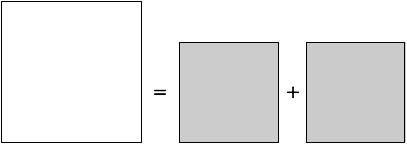
\includegraphics[scale=0.4]{FiguresArithmetic/sqrt2initial}
\caption{{\it A geometric depiction of the Pythagorean Theorem and its
    underlying equation: $a^2 = b^2 + b^2$.}
\label{fig:irrationality1}}
\end{center}
\end{figure}
suggestively invokes the Pythagorean Theorem.  The figure displays three squares: The two small grey squares are identical, with common area $A$, while the large white square has double this area.  By the Pythagorean Theorem, if the small squares have (common) side-lengths $b \in \N^+$, hence share area $A = b^2$ each, then the large square has side-lengths $a \eqdef \sqrt{2}b$, hence has area $a^2 = 2 b^2$.

As in the classical proof of Section~\ref{sec:classical-proof-sqrt(2)}, we now assume that $\sqrt{2}$ is rational.  Within the context of Fig.~\ref{fig:irrationality1}, this means that
\[ \sqrt{2} \ = \ {a \over b} \]
for $a, b \in \N^+$.  Since all that we have said thus far holds for arbitrary $a$ and $b$, we are free to insist, as before, that $a$ and $b$ do not share any common prime factor.  Note additionally that because\footnote{If this inequality is new to you, then just note that $(1.4)^2 = 1.96$, which is less than $2$.}
\[ \sqrt{2} \ > \ 1.4 \]
we know that $a > b$.

\bigskip

\noindent \fbox{
\begin{minipage}{0.96\textwidth}
{\bf Explanatory note}.

\smallskip

Of course, our demand that the numerator $a$ and the denominator $b$ do not share a common factor does not diminish the generality of our argument.  This is because ``$a/b$'' is just one name for the depicted rational number, and choosing any specific name has no impact on the number itself.
\end{minipage}
}
\bigskip

Now that we have the suggestive ``equation'' presented in Fig.~\ref{fig:irrationality1}, we can manipulate the depicted squares.  We embed both of the grey $b \times b$ squares of
Fig.~\ref{fig:irrationality1} into the white $a \times a$ square, in the overlapped manner depicted in Fig.~\ref{fig:irrationality2}:
\begin{figure}[htb]
\begin{center}
       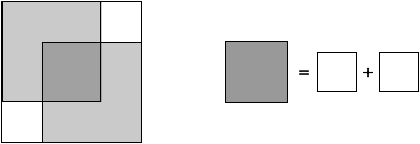
\includegraphics[scale=0.4]{FiguresArithmetic/sqrt2final}
\caption{{\it Constructing a smaller instance of the Pythagorean equation.}
\label{fig:irrationality2}}
\end{center}
\end{figure}
one grey square is nestled into the northwestern corner of the white square, while the other is nestled into the southeastern corner.  The overlapping of the grey squares under this embedding creates a new square---depicted in dark grey---in the center of the white square, while it leaves unoccupied two small squares, which remain white in the figure.

\smallskip

Now, let us get quantitative.
\begin{itemize}
\item
On the one hand, the fact that the combined areas of the two grey squares equal the area of the white square guarantees that the area of the dark grey overlap-square is equal to the combined areas of the small unoccupied white squares.

\medskip\item
On the other hand, because the side-length of the large white square is $a$, while the (common) side-length of the grey squares is $b$, it follows that the side-lengths of the small white square is $a-b$, and the side-length of the dark grey overlap-square is $2b-a$.  All of these side-lengths are positive because of the value of $\sqrt{2}$.  To wit: ($i$) $a > b$ because $\sqrt{2} >1$; ($ii$) $2b >a$ because $\sqrt{2} < 2$.
\end{itemize}
The preceding facts allow us to label the squares of Fig.~\ref{fig:irrationality1} differently than we did earlier---and thereby derive a different valid ``equation''.  As we did at the beginning of this discussion, we again invoke the Pythagorean Theorem, but now we do so while focusing---cf., Fig.~\ref{fig:irrationality2}---on the dark grey overlap-square (which plays the role of the large square in Fig.~\ref{fig:irrationality1}) and the two small white squares (which play the role of the two small squares in Fig.~\ref{fig:irrationality1}).  Whereas our original focus led to the putative rational value for $\sqrt{2}$: $\displaystyle {a \over b}$ for $\sqrt{2}$, the new focus yields the putative rational value $\displaystyle {2b-a \over a-b}$.  We thus have
\[ \sqrt{2} \ = \ {a \over b} \ = \ {2b-a \over a-b}, \]
where $2b-a \ < \ a$ and $a-b \ < \ b$.  In the light of the Fundamental Theorem of Arithmetic (Theorem~\ref{thm:Fund-Thm-Arith}), this new rational name for $\sqrt{2}$ contradicts our initial assumption that $a/b$ was a fraction {\em in lowest  terms}, i.e., in which $a$ and $b$ share no common factor.  \qed
\end{proof}

\index{fraction in {\em lowest terms}}

\section{The Basics of the Complex Numbers}
\label{sec:complexes}

\index{number!complex!real part} \index{$i$: the imaginary unit}
\index{number!complex!imaginary part} \index{imaginary unit $i$}
Let us denote by $\C$ the set of complex numbers.  Each number $\kappa = a+bi$ in $\C$ has a {\it real}  {\em part}---the part that {\em does not} involve the imaginary unit $i$---and an {\it imaginary} {\em part}---the part that {\em does} involve $i$.  To be explicit: the real part of our number $\kappa$, is Re$(\kappa) = a$; the {\it imaginary part} of our number $\kappa$ is Im$(\kappa) = b$.  The notations Re$(\kappa)$ and Im$(\kappa)$ are common but not universal.
\index{complex number!imaginary part Im($\cdot$)} 
\index{complex number!imaginary part Im($\cdot$)} 
\index{complex number!real part Re($\cdot$)}

\medskip

\index{complex number!multiplication!three real multiplications}
Based on the arithmetic laws that we have discussed thus far, plus the defining equation ($i^2 = -1$) of the imaginary unit $i$, we find that the {\em product} of two complex numbers, $a+bi \in \C$ and $c+di \in \C$ is the complex number
\begin{equation}
\label{eq:complex-mult}
(a+bi) \cdot (c+di) \ = \ (ac - bd) + (ad + bc)i
\end{equation}
We note that a ``direct'' implementation of complex multiplication, i.e., one that implements Eq.~(\ref{eq:complex-mult}) literally, requires {\em four} real multiplications---namely, $a \times c, \ b \times d, \ a \times d, \ b \times c$.

During the 1960s, people began to pay close attention to the differing costs associated with alternative ways of achieving computational results.  They sought---and found---a number of procedures that replaced computations involving $k$ real multiplications (a relatively expensive operation) and $\ell$ real additions (a relatively inexpensive operation) by computations that achieved the same result but used fewer multiplications and not too many more additions. Complex multiplication was one of the operations they studied.  Here is the result.

\begin{prop}
\label{thm:complex-mult-3real}
One can compute the product of two complex numbers using {\em three} real multiplications rather than four.
\end{prop}

The proof of this result involves arithmetic manipulation that requires ``thinking outside the box".  
We leave the proof as an exercise.  The main message of the result is that we should never be lulled into assuming that the way an arithmetic expression {\em is} written is the way that it {\em has to be} written.


%%%%%%%%%%%%%%%%%%%%%%%%%%%%%%%%%%%%%%%%%%%%%%%%%%%

\section{Exercises: Chapter 4}

Throughout the text, we mark each exercise with 0 or 1 or 2 occurrences of the symbol $\oplus$, as a rough gauge of its level of challenge.  The 0-$\oplus$ exercises should be accessible by just reviewing the text.  We provide {\em hints} for the 1-$\oplus$ exercises; Chapter~\ref{ch:Exercises} provides {\em solutions} for the 2-$\oplus$ exercises.  Additionally, we begin each exercise with a brief explanation of its anticipated value to the reader. 


\begin{enumerate}
\item
{\bf Irrationality abounds!}

{\sc Lesson:} Extending an argument by understanding its basis.

\smallskip

{\em Extend Euclid's reasoning about $\sqrt{2}$ to prove the following assertion.}

\index{$\sqrt{p}$ is irrational for any prime $p$}

\begin{prop}
For any prime $p >1$, the number $\sqrt{p}$ is not rational, i.e., does not belong to $\Q$.
\end{prop}

\medskip\item
{\bf Appreciating the totality of algebra}

{\em Lesson:} Even if a problem does not mention the inverses to addition and multiplication, you may benefit from paying attention to these operations.

\smallskip

\index{complex number!multiplication via 3 real multiplications}

{\em Show how to compute the product of two complex numbers using only {\em three}
real multiplications rather than the method that directly follows the definition (which uses four multiplications).}\footnote{Make a note of your solution technique.  We shall encounter it again in Chapter~\ref{ch:Recurrences}.}

\bigskip

\noindent \fbox{
\begin{minipage}{0.96\textwidth}
Of course, a full reckoning of the comparative costs of multiplying complex numbers using three real multiplications vs.~four must consider that the $3$-multiplication procedure uses {\em three} real additions, whereas the $4$-multiplication procedure uses only {\em two} real additions.  A complete comparison between the two procedures would require knowing the relative costs of multiplication and addition on the target computing platform.
\end{minipage}
}
\medskip

\medskip\item
{\bf Basic properties of divisibility}

{\sc Lessons:} Practice with basic proofs; enhance understanding of integers

\smallskip

{\em Prove the four assertions in Proposition~\ref{thm:basic-divisibility}}.
\smallskip

\medskip\item
{\bf Observing an influence of parity}

{\em Lesson:} Learn to recognize the influence of numerical properties such as parity whenever one deals with sequences of numbers.

\smallskip

The notion of even-odd parity is so simple that one often overlooks the way it can influence the ``shape" of computations.  You will now observe such influence on the important area of {\em recurrences}.  We shall study recurrent summations in depth in Chapter~\ref{ch:Recurrences} and in Appendix~\ref{ch:recurrent-numbers-appendix}, but we begin this study with the simple topic of this exercise.

\medskip

It is not uncommon, in mathematics, computing, and allied disciplines, to encounter sequences of integers that have recursive structures that are kindred to the following sequences:
\begin{itemize}
\item
{\em A bilinear recurrence}
\begin{equation}
\label{eq:bilinear-seqspec}
\begin{array}{ll}
\mbox{Two base integers:} & a_0, \ a_1 \\
\mbox{The recurrent remainder:} &
(\forall n \geq 1) \ \big[ a_{n+1} \ = \ a_n + a_{n-1} \big]
\end{array}
\end{equation}

\medskip\item
{\em A trilinear recurrence}
\begin{equation}
\label{eq:trilinear-seqspec}
 \begin{array}{ll}
\mbox{Three base integers:} & b_0, \ b_1, \ b_2 \\
\mbox{The recurrent remainder:} &
(\forall n \geq 1) \ \big[ b_{n+1} \ = \ b_n + b_{n-1} + b_{n-2} \big]
\end{array}
\end{equation}
\end{itemize}
Viewing these specifications inductively, formulas (\ref{eq:bilinear-seqspec}) and (\ref{eq:trilinear-seqspec}) generate two infinite sequence of positive integers:
\[ a_0, a_1, a_2, a_3, a_4, \ldots \ \ \ \mbox{ and } \ \ \ b_0, b_1, b_2, b_3, b_4, \ldots \]
We are interested in exposing some properties of these sequences that are consequences of the parities of their respective base integers.

\smallskip
On to the exercise:

\medskip

Of course, if one chooses only even positive base integers, then the entire sequence $A$ generated by formula (\ref{eq:bilinear-seqspec}) and the entire sequence $B$ generated by formula (\ref{eq:trilinear-seqspec}) consist of even integers.

{\it Answer the following questions for each of these sequences.}
  \begin{enumerate}
  \item
{\em Is there a choice of positive base integers $a_0, \ a_1$ for which the entire sequence $A$ consists of only odd integers?}
  \medskip\item
{\em Is there a choice of positive base integers $b_0, \ b_1, \ b_2$ for which the entire sequence $B$ consists of only odd integers?}
  \medskip\item
{\em Is there a choice of positive base integers $a_0, \ a_1$ for which the entire sequence $A$ alternates between even and odd integers?}
  \medskip\item
{\em Is there a choice of positive base integers $b_0, \ b_1, \ b_2$ for which the entire sequence $B$  alternates between even and odd integers?}
\end{enumerate}

\medskip\item
$\oplus$ {\bf The rationals ($\Q$) and the integers ($\N$) are equinumerous}

{\sc Lesson:} Experience with a ``multilayer" proof, which combines several elementary threads

\smallskip

{\em Provide a {\em detailed} proof of Proposition~\ref{thm:|Q|=|N|}.}  Informally, there are equally many integers as there are rationals.
\end{enumerate}

\ignore{*********************
\subsection{Another proof for irrationality of $\sqrt{2}$}

\noindent \textit{The aim.}
Reenforcing the ability of using geometrical proofs.
\medskip

\noindent \textit{The problem.}
Prove the irrationality of $\sqrt{2}$ using a geometrical argument.
\medskip

\noindent \textit{Hint.}
The proof is by contradiction. 

Consider $\sqrt{2}$ is rational, which means there exists a pair of integers $(a,b)$
such that $\sqrt{2} = \frac{a}{b}$ (where $a$ is larger than $b$).
Represent this expression geometrically by the corresponding isosceles right triangle
which is the one of minimal surface. 
%The contradiction comes by constructing another isosceles triangle with a smaller surface.
%Squaring this expression leads to $2.b^2 = a^2$.
\medskip

\noindent \textit{Lesson learned.}
Experiencing a proof which uses two types of arguments (contradiction and geometrical figure).


\begin{proof}
Although implementing Eq.~(\ref{eq:complex-mult}) ``directly'' correctly
produces the product $\kappa = (a+bi) \cdot (c+di)$, there is another
implementation that is {\em more efficient}.  Specifically, the
following recipe computes $\kappa$ using only {\em three} real
multiplications instead of the four real multiplications of the
``direct'' implementation.  We begin to search for this recipe by
noting that our immediate goal is to compute both Re$(\kappa) = ac-bd$
and Im$(\kappa) = ad+bc$.  We can accomplish this by computing the
{\em three} real products
\begin{equation}
\label{eq:complex-mult-3a}
(a+b) \cdot (c+d); \ \ \ \ \
ac;  \ \ \ \ \ bd
\end{equation}
and then noting that
\begin{equation}
\label{eq:complex-mult-3b}
\begin{array}{lcl}
\mbox{Im}(\kappa) & = & (a+b) \cdot (c+d) - ac -bd, \\
\mbox{Re}(\kappa) & = & ac -bd
\end{array}
\end{equation}
We thereby achieve the result of the complex multiplication described
in Eq.~(\ref{eq:complex-mult}) while using only {\em three} real
multiplications.

Of course, a full reckoning of the costs of the two implementations we
have discussed exposes the fact that the implementation that invokes
Eqs.~(\ref{eq:complex-mult-3a}) and (\ref{eq:complex-mult-3b}) uses {\em
  three} real additions rather than the {\em two} real additions of
the ``direct'' implementation.  But this entire exercise was
predicated on the observation that each real addition is much less
costly than a real multiplication, so trading one multiplication for
one addition is an unqualified ``win''.  \qed
\end{proof}

{\Denis I added a sentence to refer to an exercice dealing with karatsuba which uses the same idea...}
Notice that this technique is classical and it has been used in many other situations.
For instance while multiplying two integers in base 2 (see exercice~\ref{Karatsuba}).

*******************}
